\documentclass{standalone}
\usepackage{tikz}
\usetikzlibrary{patterns, positioning}


\begin{document}
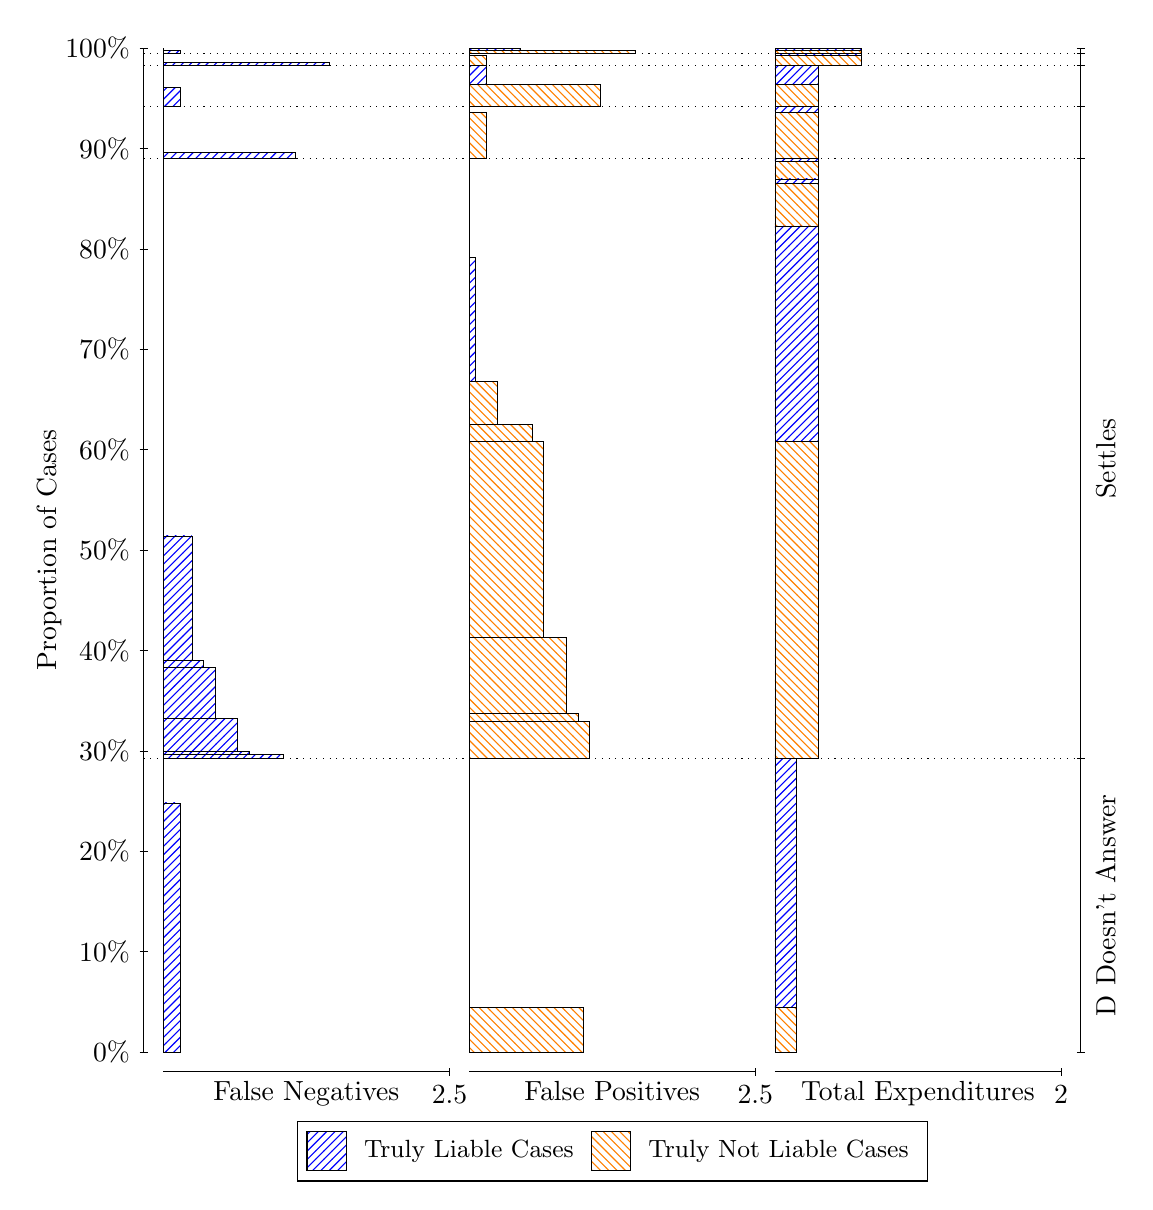
\begin{tikzpicture}
\draw[black, very thin] (1.5,1.75) -- (1.5,14.5);
\node[rotate=90, text=black, anchor=center] at (0.3, 8.125) {Proportion of Cases};
\draw[black, very thin] (1.45,1.75) -- (1.55,1.75);
\node[text=black, anchor=east] at (1.45, 1.75) {0\%};
\draw[black, very thin] (1.45,3.025) -- (1.55,3.025);
\node[text=black, anchor=east] at (1.45, 3.025) {10\%};
\draw[black, very thin] (1.45,4.3) -- (1.55,4.3);
\node[text=black, anchor=east] at (1.45, 4.3) {20\%};
\draw[black, very thin] (1.45,5.575) -- (1.55,5.575);
\node[text=black, anchor=east] at (1.45, 5.575) {30\%};
\draw[black, very thin] (1.45,6.85) -- (1.55,6.85);
\node[text=black, anchor=east] at (1.45, 6.85) {40\%};
\draw[black, very thin] (1.45,8.125) -- (1.55,8.125);
\node[text=black, anchor=east] at (1.45, 8.125) {50\%};
\draw[black, very thin] (1.45,9.4) -- (1.55,9.4);
\node[text=black, anchor=east] at (1.45, 9.4) {60\%};
\draw[black, very thin] (1.45,10.675) -- (1.55,10.675);
\node[text=black, anchor=east] at (1.45, 10.675) {70\%};
\draw[black, very thin] (1.45,11.95) -- (1.55,11.95);
\node[text=black, anchor=east] at (1.45, 11.95) {80\%};
\draw[black, very thin] (1.45,13.225) -- (1.55,13.225);
\node[text=black, anchor=east] at (1.45, 13.225) {90\%};
\draw[black, very thin] (1.45,14.5) -- (1.55,14.5);
\node[text=black, anchor=east] at (1.45, 14.5) {100\%};

\draw[black, very thin] (13.4,1.75) -- (13.4,14.5);
\draw[black, very thin] (13.35,1.75) -- (13.45,1.75);
\node[anchor=west] at (13.35, 1.75) {};
\draw[black, very thin] (13.35,5.4762) -- (13.45,5.4762);
\node[anchor=west] at (13.35, 5.4762) {};
\draw[black, very thin] (13.35,13.096) -- (13.45,13.096);
\node[anchor=west] at (13.35, 13.096) {};
\draw[black, very thin] (13.35,13.763) -- (13.45,13.763);
\node[anchor=west] at (13.35, 13.763) {};
\draw[black, very thin] (13.35,14.282) -- (13.45,14.282);
\node[anchor=west] at (13.35, 14.282) {};
\draw[black, very thin] (13.35,14.435) -- (13.45,14.435);
\node[anchor=west] at (13.35, 14.435) {};
\draw[black, very thin] (13.35,14.5) -- (13.45,14.5);
\node[anchor=west] at (13.35, 14.5) {};

\draw[black, very thin, pattern color=blue, pattern=north east lines] (1.75,1.75) rectangle (1.968,4.9142);
\draw[black, very thin, pattern color=orange, pattern=north west lines] (1.75,4.9142) rectangle (1.75,5.4762);
\draw[black, very thin, pattern color=blue, pattern=north east lines] (1.75,5.4762) rectangle (3.276,5.5309);
\draw[black, very thin, pattern color=blue, pattern=north east lines] (1.75,5.5309) rectangle (2.84,5.5654);
\draw[black, very thin, pattern color=blue, pattern=north east lines] (1.75,5.5654) rectangle (2.6947,5.9875);
\draw[black, very thin, pattern color=blue, pattern=north east lines] (1.75,5.9875) rectangle (2.404,6.6347);
\draw[black, very thin, pattern color=blue, pattern=north east lines] (1.75,6.6347) rectangle (2.2587,6.7272);
\draw[black, very thin, pattern color=blue, pattern=north east lines] (1.75,6.7272) rectangle (2.1133,8.3056);
\draw[black, very thin, pattern color=orange, pattern=north west lines] (1.75,8.3056) rectangle (1.75,13.096);
\draw[black, very thin, pattern color=blue, pattern=north east lines] (1.75,13.096) rectangle (3.4213,13.172);
\draw[black, very thin, pattern color=orange, pattern=north west lines] (1.75,13.172) rectangle (1.75,13.763);
\draw[black, very thin, pattern color=blue, pattern=north east lines] (1.75,13.763) rectangle (1.968,14.002);
\draw[black, very thin, pattern color=orange, pattern=north west lines] (1.75,14.002) rectangle (1.75,14.282);
\draw[black, very thin, pattern color=blue, pattern=north east lines] (1.75,14.282) rectangle (3.8573,14.314);
\draw[black, very thin, pattern color=orange, pattern=north west lines] (1.75,14.314) rectangle (1.75,14.435);
\draw[black, very thin, pattern color=blue, pattern=north east lines] (1.75,14.435) rectangle (1.968,14.468);
\draw[black, very thin, pattern color=orange, pattern=north west lines] (1.75,14.468) rectangle (1.75,14.5);
\draw[black, very thin, pattern color=orange, pattern=north west lines] (5.6333,1.75) rectangle (7.0867,2.312);
\draw[black, very thin, pattern color=blue, pattern=north east lines] (5.6333,2.312) rectangle (5.6333,5.4762);
\draw[black, very thin, pattern color=orange, pattern=north west lines] (5.6333,5.4762) rectangle (7.1593,5.9525);
\draw[black, very thin, pattern color=orange, pattern=north west lines] (5.6333,5.9525) rectangle (7.014,6.0524);
\draw[black, very thin, pattern color=orange, pattern=north west lines] (5.6333,6.0524) rectangle (6.8687,7.0174);
\draw[black, very thin, pattern color=orange, pattern=north west lines] (5.6333,7.0174) rectangle (6.578,9.5008);
\draw[black, very thin, pattern color=orange, pattern=north west lines] (5.6333,9.5008) rectangle (6.4327,9.7241);
\draw[black, very thin, pattern color=orange, pattern=north west lines] (5.6333,9.7241) rectangle (5.9967,10.266);
\draw[black, very thin, pattern color=blue, pattern=north east lines] (5.6333,10.266) rectangle (5.706,11.845);
\draw[black, very thin, pattern color=blue, pattern=north east lines] (5.6333,11.845) rectangle (5.6333,13.096);
\draw[black, very thin, pattern color=orange, pattern=north west lines] (5.6333,13.096) rectangle (5.8513,13.687);
\draw[black, very thin, pattern color=blue, pattern=north east lines] (5.6333,13.687) rectangle (5.6333,13.763);
\draw[black, very thin, pattern color=orange, pattern=north west lines] (5.6333,13.763) rectangle (7.3047,14.042);
\draw[black, very thin, pattern color=blue, pattern=north east lines] (5.6333,14.042) rectangle (5.8513,14.282);
\draw[black, very thin, pattern color=orange, pattern=north west lines] (5.6333,14.282) rectangle (5.8513,14.402);
\draw[black, very thin, pattern color=blue, pattern=north east lines] (5.6333,14.402) rectangle (5.6333,14.435);
\draw[black, very thin, pattern color=orange, pattern=north west lines] (5.6333,14.435) rectangle (7.7407,14.466);
\draw[black, very thin, pattern color=blue, pattern=north east lines] (5.6333,14.466) rectangle (6.2873,14.5);
\draw[black, very thin, pattern color=orange, pattern=north west lines] (9.5167,1.75) rectangle (9.7892,2.312);
\draw[black, very thin, pattern color=blue, pattern=north east lines] (9.5167,2.312) rectangle (9.7892,5.4762);
\draw[black, very thin, pattern color=orange, pattern=north west lines] (9.5167,5.4762) rectangle (10.062,9.5008);
\draw[black, very thin, pattern color=blue, pattern=north east lines] (9.5167,9.5008) rectangle (10.062,12.241);
\draw[black, very thin, pattern color=orange, pattern=north west lines] (9.5167,12.241) rectangle (10.062,12.783);
\draw[black, very thin, pattern color=blue, pattern=north east lines] (9.5167,12.783) rectangle (10.062,12.838);
\draw[black, very thin, pattern color=orange, pattern=north west lines] (9.5167,12.838) rectangle (10.062,13.061);
\draw[black, very thin, pattern color=blue, pattern=north east lines] (9.5167,13.061) rectangle (10.062,13.096);
\draw[black, very thin, pattern color=orange, pattern=north west lines] (9.5167,13.096) rectangle (10.062,13.687);
\draw[black, very thin, pattern color=blue, pattern=north east lines] (9.5167,13.687) rectangle (10.062,13.763);
\draw[black, very thin, pattern color=orange, pattern=north west lines] (9.5167,13.763) rectangle (10.062,14.042);
\draw[black, very thin, pattern color=blue, pattern=north east lines] (9.5167,14.042) rectangle (10.062,14.282);
\draw[black, very thin, pattern color=orange, pattern=north west lines] (9.5167,14.282) rectangle (10.607,14.402);
\draw[black, very thin, pattern color=blue, pattern=north east lines] (9.5167,14.402) rectangle (10.607,14.435);
\draw[black, very thin, pattern color=orange, pattern=north west lines] (9.5167,14.435) rectangle (10.607,14.466);
\draw[black, very thin, pattern color=blue, pattern=north east lines] (9.5167,14.466) rectangle (10.607,14.5);
\draw[black, dotted] (1.5,5.4762) -- (13.4,5.4762);
\draw[black, dotted] (1.5,13.096) -- (13.4,13.096);
\draw[black, dotted] (1.5,13.763) -- (13.4,13.763);
\draw[black, dotted] (1.5,14.282) -- (13.4,14.282);
\draw[black, dotted] (1.5,14.435) -- (13.4,14.435);
\draw[black, very thin] (1.75,1.5) -- (5.3833,1.5);
\node[text=black, anchor=north] at (3.5667, 1.5) {False Negatives};
\draw[black, very thin] (5.3833,1.45) -- (5.3833,1.55);
\node[text=black, anchor=north] at (5.3833, 1.45) {2.5};

\draw[black, very thin] (5.6333,1.5) -- (9.2667,1.5);
\node[text=black, anchor=north] at (7.45, 1.5) {False Positives};
\draw[black, very thin] (9.2667,1.45) -- (9.2667,1.55);
\node[text=black, anchor=north] at (9.2667, 1.45) {2.5};

\draw[black, very thin] (9.5167,1.5) -- (13.15,1.5);
\node[text=black, anchor=north] at (11.333, 1.5) {Total Expenditures};
\draw[black, very thin] (13.15,1.45) -- (13.15,1.55);
\node[text=black, anchor=north] at (13.15, 1.45) {2};

\node[text=black, centered, rotate=90] at (13.72, 3.6131) {D Doesn't Answer};
\node[text=black, centered, rotate=90] at (13.72, 9.286) {Settles};





\draw (7.449999999999999,1.5) node[draw=none] (baseCoordinate) {};
\begin{scope}[align=center]
        \matrix[scale=0.5, draw=black, below=0.5cm of baseCoordinate, nodes={draw}, column sep=0.1cm]{
            \node[rectangle, draw, minimum width=0.5cm, minimum height=0.5cm, pattern color=blue, pattern=north east lines] {}; &
            \node[draw=none, font=\small, text=black] (B) {Truly Liable Cases}; &
            \node[rectangle, draw, minimum width=0.5cm, minimum height=0.5cm, pattern color=orange, pattern=north west lines] {}; &
            \node[draw=none, font=\small, text=black] (B) {Truly Not Liable Cases}; \\
            };
\end{scope}

\end{tikzpicture}
\end{document}